
% VLDB template version of 2020-08-03 enhances the ACM template, version 1.7.0:
% https://www.acm.org/publications/proceedings-template
% The ACM Latex guide provides further information about the ACM template

\documentclass[sigconf, nonacm]{acmart}

%% The following content must be adapted for the final version
% paper-specific
\newcommand\vldbdoi{XX.XX/XXX.XX}
\newcommand\vldbpages{XXX-XXX}
% issue-specific
\newcommand\vldbvolume{14}
\newcommand\vldbissue{1}
\newcommand\vldbyear{2020}
% should be fine as it is
\newcommand\vldbauthors{\authors}
\newcommand\vldbtitle{\shorttitle} 
% leave empty if no availability url should be set
\newcommand\vldbavailabilityurl{URL_TO_YOUR_ARTIFACTS}
% whether page numbers should be shown or not, use 'plain' for review versions, 'empty' for camera ready
\newcommand\vldbpagestyle{plain} 

\usepackage{algorithm} 
\usepackage{algpseudocode}
\usepackage{listings}
\usepackage{xcolor} 

% 定义代码样式
\lstset{
    language=C++, 
    basicstyle=\ttfamily\small, % 设置基本字体
    keywordstyle=\color{blue}, % 关键字颜色
    commentstyle=\color{green}, % 注释颜色
    stringstyle=\color{red}, % 字符串颜色
    numbers=left, % 显示行号
    numberstyle=\tiny\color{gray}, % 行号样式
    breaklines=true, % 自动换行
    frame=single, % 添加边框
    captionpos=b, % 标题位置(底部)
    tabsize=4 % 设置制表符宽度
}

\begin{document}
\title{The Design and Optimization of High Performance Approximate Nearest Neighbor Algorithm}

%%
%% The "author" command and its associated commands are used to define the authors and their affiliations.
\author{Yiwei Zhang}
\affiliation{%
  \institution{Acabridge Academy Shanghai}
  \city{Shanghai}
  \country{China}
}
\email{aaron.zhang.me@qq.com}

%%
%% The abstract is a short summary of the work to be presented in the
%% article.
\begin{abstract}
With the widespread use of Large Language Model (LLM) and Retrieval Augmented Generation (RAG), vector search of high efficiency and low cost has become a key requirement. HNSW (Hierarchical Navigable Small World) becomes a popular Approximate Nearest Neighbor (ANN) algorithm because of its high recall rate.  However, the practical application of the ANN algorithm is limited due to its high memory usage and computational latency.  
This paper proposes an enhancement on the HNSW algorithm based on locally adaptive vector quantization (HNSW-LVQ), which significantly reduces memory overhead and accelerates distance computation by per-dimension quantization that compresses floating-point vector to integer representations.
Experiments show that on the SIFT\_10K dataset, the average query latency of HNSW-LVQ is significantly reduced by 85\% (from 0.844 to 0.124 seconds) with a mere 2\% drop in the recall rate (from 100\% to 98\%), while its memory usage is greatly enhanced.  This paper verifies the effectiveness of integrating quantization techniques into graph indexing, providing a feasible optimization direction for industrial-grade vector databases.  Future research work will expand to larger datasets and explore residual quantization to further improve accuracy and efficiency.

\end{abstract}

\maketitle

%%% do not modify the following VLDB block %%
%%% VLDB block start %%%
\pagestyle{\vldbpagestyle}
%%% VLDB block end %%%


\section{Introduction}

Vector search, a cornerstone of modern information retrieval, enables rapid similarity comparisons in high-dimensional spaces through metrics like Euclidean distance and cosine similarity.  Nowadays, Large Language Models (LLMs) and Retrieval Augmented Generation (RAG) \cite{lewis2020retrieval} systems are widely deployed in industrial scenarios where vector search plays an important role in bridging the static knowledge bases and dynamic user queries. In RAG frameworks, vector search retrieves semantically relevant documents from a vast collection of information to provide contexts for LLM responses. It enables models to address domain-specific questions with unprecedented accuracy in cases like enterprise data queries or medical literature analysis. For instance, platforms like ChatGPT rely on vector search to integrate proprietary databases, ensuring responses adhere to organizational knowledge while mitigating deviations. However, this capability relies on the efficiency of Approximate Nearest Neighbor (ANN) algorithms, which face increasing demands as data scales into billions of dimensions across industries like e-commerce, genomics, and autonomous systems.

The brute-force approach, exhaustively comparing a query vector against all stored vectors, guarantees perfect recall results, but becomes computational costly for datasets exceeding millions of entries. ANN algorithms, however, address this by trading marginal recall losses for tremendous speed accerlations. Among these, graph-based Hierarchical Navigable Small World (HNSW) has emerged as a gold standard due to its exceptional balance between recall and speed. HNSW constructs a multi-layered graph where upper layers enable long-range "hops" for coarse exploration, while lower layers refine searches through localized connections. This hierarchical design, inspired by skip lists and small-world networks, achieves logarithmic search complexity, outperforming alternatives like IVF (Inverted File) in recall rates. For example, on the BigANN benchmark, HNSW consistently delivers >95\% recall at sub-millisecond latencies for moderate-sized datasets.

Despite its strengths, HNSW faces two critical limitations in industrial implementations. First, its memory footprint grows linearly with dataset size, as raw vectors and multi-layer adjacency lists must reside in memory. A billion-scale HNSW index can exceed 1TB, straining hardware budgets and limiting cloud deployment flexibility. Second, distance calculations between high-dimensional vectors dominate computational latency. Each 128-dimensional Euclidean distance computation requires 128 floating-point operations (multiplications and additions), consuming about 50\% of total query time in CPU-bound systems. These challenges are worsened in real-time applications, such as recommendation engines or fraud detection, where latency spikes directly impact user experience or operational costs.

This paper proposes HNSW-LVQ (Locally Adaptive Vector Quantization enhanced HNSW), a novel optimization framework that tackles both memory and computational bottlenecks. Unlike global quantization methods like Product Quantization (PQ), which apply uniform compression across all vectors, LVQ customizes quantization parameters per dimension. By analyzing the value distribution of each dimension (e.g., via min-max scaling), LVQ compresses 32-bit floats into 8-bit integers with minimal precision loss. This reduces vector storage by 75\% and replaces floating-point arithmetic with integer operations during graph traversal, accelerating distance calculations. Crucially, LVQ’s per-dimension adaptability preserves local data distributions, mitigating the "quantization cliffs" observed in PQ when subspaces exhibit skewed value ranges.

My design and enhancement of the ANN algorithm is characterized by the following:

\begin{enumerate}
    \item Algorithmic Innovation: LVQ is integrated into HNSW’s indexing and search pipelines, which demonstrates compatibility with graph-based ANN without sacrificing hierarchical navigability.
    \item Empirical Validation: On the SIFT\_10K dataset, HNSW-LVQ reduces average query latency by 85\% (from 0.844 seconds to 0.124 seconds) with a negligible 2\% recall drop (100\% → 98\%).
    \item Industrial Relevance: The work provides a blueprint for hybrid graph-quantization architectures, addressing scalability barriers in vector databases like Milvus and Qdrant.
\end{enumerate}

The remainder of this paper is structured as follows: 
\begin{enumerate}
    \item Section 2 reviews ANN algorithms and quantization techniques;
    \item Section 3 details HNSW-LVQ’s design and implementation; 
    \item Section 4 evaluates performance against baselines;
    \item Section 5 discusses future directions and potential improvements;
    \item Section 6 is the dissertation review.
\end{enumerate}
By integrating adaptive compression into graph indexing, this research explores the feasibility of billion-scale vector search in resource-constrained environments.
 

\section{Literature Review}

Approximate Nearest Neighbor (ANN) search has emerged as a cornerstone of modern data retrieval systems, driven by the exponential growth of high-dimensional data in applications ranging from artificial intelligence to real-time recommendation engines. This section provides a complete analysis of ANN methodologies, covering classical algorithms, cutting-edge innovations, and interdisciplinary approaches, while critically evaluating their theoretical underpinnings, practical tradeoffs, and scalability in industrial settings. 

\subsection{Inverted File (IVF) and Its Variants}
Inverted File (IVF) structures \cite{invertedindex} are foundational to ANN algorithms, inspired by their success in text retrieval systems. In ANN, datasets are separated into K subspaces (clusters) using clustering algorithms like K-means\cite{kmeans}. Each cluster is associated with an inverted list containing vectors assigned to it. During retrieval, the query vector is first compared to cluster centroids to identify the nearest nprobe clusters, followed by exhaustive searches within these clusters.

Advancements on IVF and its variants include: 
\begin{enumerate}
    \item GPU Acceleration: Frameworks like Faiss\cite{johnson2019billion} from Facebook leverage GPU parallelism to accelerate clustering and distance computations, enabling IVF to handle billion-scale datasets efficiently. For instance, IVFFlat in Faiss achieves high throughput by offloading brute-force comparisons to GPU cores.
    \item Dynamic Load Balancing: SPANN \cite{chen2021spann} introduces hierarchical clustering combined with Principal Component Analysis (PCA) \cite{pca} for dimensionality reduction. By dynamically redistributes vectors across clusters based on access patterns, SPANN minimizes disk I/O overhead in distributed systems. 
	\item Adaptive nprobe Optimization: Modern implementations dynamically adjust nprobe (the number of clusters probed) during queries. For example, nprobe can be adapted based on query complexity or real-time latency constraints, balancing recall and speed.
\end{enumerate}

Limitations on IVF based methods include:

\begin{enumerate}
    \item Cluster Boundary Sensitivity: IVF’s recall heavily depends on clustering quality. Queries near cluster boundaries risk missing true nearest neighbors, especially when data distributions are non-uniform. 
    \item Memory-Throughput Tradeoff: While IVF reduces memory usage by storing only centroids and inverted lists, large K values (for finer granularity) increase centroid storage overhead and clustering time.
\end{enumerate}

In summary, IVF-based ANN algorithms have advantages in low memory usage (storing only cluster centers and inverted lists) and fast retrieval speed, but they suffer from recall sensitivity to clustering quality. If the query vector lies at the intersection of multiple clusters, it may potentially miss some nearest neighbors near cluster boundaries.

\subsection{Product Quantization (PQ) and Hybrid Methods}
Product Quantization (PQ) \cite{johnson2019billion} revolutionized ANN by compressing high-dimensional vectors into compact codes. PQ splits a D-dimensional vector into M subvectors, each quantized using a pre-trained codebook. The original vector is represented by M codeword indices, reducing storage from 4D bytes (float32) to M bytes (e.g., 8 bytes for M=8). During queries, distances are approximated using precomputed lookup tables.

Combining IVF with PQ (e.g., IVF-PQ in Faiss) achieves a favorable tradeoff. IVF reduces the search space, while PQ accelerates distance calculations. For example, PQ-8×8 compresses 128D vectors to 8 bytes, enabling efficient billion-scale searches on GPUs.

However, while Product Quantization (PQ) enhances performance and reduces memory costs, it also faces challenges. Specifically, PQ introduces quantization errors due to its uniform subspace partitioning, which overlooks the intra-subspace data distributions. This results in information loss and, consequently, a decrease in the recall rate of ANN search. If we apply 1-bit Product Quantization, it essentially becomes binary quantization. While this approach further compresses vectors, it also suffers from higher approximation errors. There are some works to resolve the PQ challenges:
\begin{enumerate}
    \item Residual Quantization (RQ)\cite{aguerrebere2023similarity} addresses quantization error by iteratively quantizing residual errors from previous stages, improving accuracy at the cost of higher memory usage.
    \item Recent work employs non-uniform codebook training. For instance, Neural Product Quantization (NPQ) \cite{guo2020accelerating} uses deep learning to learn codebooks that better preserve vector semantics.
\end{enumerate}

\subsection{Graph-Based Indexes: HNSW and Beyond}

Graph-based indexes: Graph-based indexes construct neighbor networks between vectors and use greedy search strategies for rapid nearest neighbor approximation. HNSW \cite{malkov2018efficient} is the most prominent graph index algorithm, evolving from NSW (Navigable Small World) \cite{malkov2014approximate}, as illustrated by below: \autoref{fig:hnsw}.

\begin{figure}
  \centering
  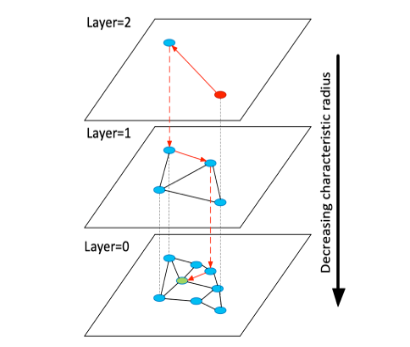
\includegraphics[width=\linewidth]{figures/hnsw.png}
  \caption{Layers of HNSW}
  \label{fig:hnsw}
\end{figure}
HNSW uses a structure similar to "probabilistic skip list" with hierarchical layers. In NSW, adding layers creates a graph with separated links across layers. The top layer has the longest links, while the bottom layer has the shortest. Starting at the top layer from the longest links, the search process moves greedily through each layer's edges until a local minimum is found. Then it shifts to a lower layer and repeats the search process until the bottom layer's local minimum is reached. 
Compared with IVF based methods, HNSW introduces several key innovations:
\begin{enumerate}
    \item  Multi-Layer Probabilistic Insertion: Vectors are randomly assigned to layers based on an exponentially decaying probability, creating a skip list-like hierarchy. This ensures logarithmic search complexity which is very useful for high performance.
    \item Dynamic Connectivity: During insertion, each node connects to M nearest neighbors in its layer, preserving the "small world" property. Parameters like efConstruction (search breadth during indexing) and M (outgoing edges per node) critically impact performance.
\end{enumerate}

Performance and limitations of HNSW:

\begin{enumerate}
    \item Recall vs. Memory: The strength of HNSW lies in its high recall rate while keeping high performance, but at the cost of high memory usage as it needs to store original vectors and multi - layer neighbor lists. For example, HNSW achieves >95\% recall on benchmarks like BigANN \cite{bigann}, but stores raw vectors and neighbor lists, leading to massive memory footprints (e.g., 1TB+ for billion-scale datasets).
    \item Optimization Frontiers: Recent work explores memory-efficient HNSW variants. For example, DiskANN\cite{jayaram2019diskann} decouples graph storage (on disk) from frequently accessed nodes (in memory), trading latency for scalability. 
\end{enumerate}

\subsection{Traditional ANN paradigms}
Locality-Sensitive Hashing (LSH)\cite{lsh} and KD-Tree\cite{kdtree} are early ANN solutions but struggle with the "curse of dimensionality." LSH hashes vectors into buckets where collisions indicate proximity. The resulting performance down grades exponentially when it comes to high dimensional data. Similarly, KD-Tree partitions space recursively along axes, becoming ineffective beyond 20 dimensions. 
In reality, ANN are long-standing algorithms.  In the past, the retrieval data used to be low dimensional, (for example, with only 10 dimensions).  Nowadays, the vector data produced by artificial intelligence usually contain tremendous high-dimensional data. A typical RAG scenario can even reach to thousands of dimensions.  That is why the traditional ANN algorithms like LSH and KD-Tree are rarely used nowadays due to their limitations on high dimensional data.

\subsection{Industrial Applications and Benchmarking}
ANN algorithms power critical applications:
\begin{enumerate}
    \item Retrieval-Augmented Generation (RAG): Systems like OpenAI’s GPT-4 use HNSW-based vector databases (e.g., Milvus \cite{milvus}) to retrieve context documents for LLMs.
    \item Recommendation Systems: Billion-scale ANN drives personalized recommendations at companies like Meta and Amazon, where IVF-PQ balances latency and accuracy.
    \item Computer Vision: Image retrieval platforms (e.g., Pinterest Visual Search\cite{pinterest}) rely on HNSW for real-time similarity matching.
Given the extensive applications of ANN, there is a wide variety of ANN algorithms. Naturally, this has led to the development of corresponding ANN benchmarks. Among these, the more prominent ones include ann-benchmark \cite{annbenchmark} and BigANN Competition \cite{bigann}, both seeing HNSW’s dominance.
\end{enumerate}


\subsection{Analysis}
IVF - based ANN algorithms (including IVF-PQ with product quantization) and graph - index - based HNSW are mainstream in vector databases \cite{vectordb}. For example, the open - source Milvus \cite{milvus} supports both IVF and HNSW algorithms, while other vector databases such as Qdrant \cite{qdrant} and Weaviate\cite{weaviate} only support HNSW implementations. In BigANN\cite{bigann} competition, regularly organized by NeruIPS, most competing projects are HNSW or its enhancements, showing its academic and industrial popularity due to higher performance and recall rate. 
Current ANN technologies are showing a trend of diversity.  As IVF and PQ methods excel in low resource consumption for super large - scale data, HNSW graph-based indexes have become the industrial mainstream with high recall rates. While HNSW and IVF-PQ represent state-of-the-art ANN algorithms, key challenges still exist:
\begin{enumerate}
    \item Memory Overhead: Graph-based methods demand excessive RAM, limiting deployment on edge devices.
    \item Dynamic Data: Most ANN indexes assume static datasets. Real-time updates (e.g., streaming data) require incremental graph/IVF updates, which are computationally expensive.
    \item Accuracy-Speed Tradeoffs: Achieving high recall on billion-scale data with low latency are always required at the same time.
\end{enumerate}

This paper focuses on the research and verification on how to enhance HNSW algorithms with quantization methodologies, so that we can achieve high recall, high performance, and low memory overhead simultaneously.

\section{Discussion and Implementation}
This paper aims to answer the question if product quantization can be integrated with HNSW as it will be extremely difficult to apply to HNSW with PQ compressing and quantifying a batch of vectors simultaneously.
\subsection{HNSW Analysis}
The Hierarchical Navigable Small World (HNSW) algorithm has become a cornerstone of graph-based Approximate Nearest Neighbor (ANN) search due to its balance of high recall and logarithmic search complexity. This section provides a granular dissection of its structural mechanics, operational workflows, and inherent limitations that necessitate optimization.

\subsubsection{Hierarchical Graph Construction}
HNSW organizes vectors into a multi-layered graph where each layer L serves distinct navigational roles. The construction begins with a probabilistic layer assignment mechanism:
\begin{displaymath}
P(L) = \frac{1}{m_l} \exp\left(-\frac{L}{m_l}\right)
\end{displaymath}

where ml (max layers) controls the decay rate. Vectors assigned to higher layers (L→ml) form sparse, long-range connections for coarse exploration, while lower layers (L→0) maintain dense, localized links for precision.
Insertion Workflow:
\begin{itemize}
    \item Layer Assignment: For a new vector q, generate a random layer using P(L).
    \item Top-Down Traversal: Starting from the highest layer ($L_{max}$), greedily search for q's nearest neighbors using a dynamic candidate list of size efConstruction.
    \item Edge Creation: In each layer >L, connect q to M nearest neighbors, pruning excess edges to preserve the "small-world" property.

\end{itemize}

Critical Parameters:
\begin{enumerate}
    \item efConstruction (exploration factor): Governs the breadth of neighbor exploration during insertion. Higher values improve graph connectivity but increase indexing time quadratically. For example, doubling efConstruction from 100 to 200 raises construction time by about 300\% on the SIFT\_1M dataset.
    \item M (maximum edges per node): Balances recall and memory. Increasing M from 12 to 16 boosts recall by 5\% but expands memory usage by 25\%.
    \item ml (max layers): Typically set to log(N), where N is the dataset size. For N=106, ml=10, but overshooting this (e.g., ml=15) introduces redundant layers, wasting 20–30\% memory.
\end{enumerate}
\subsubsection{Search Mechanics and Latency Bottlenecks}
HNSW’s search employs a hierarchical descent strategy:
\begin{itemize}
    \item Coarse-to-Fine Navigation: Start at the top layer, iteratively narrowing the candidate pool through descending layers.
    \item Greedy Traversal: At each layer, expand candidates by comparing distances to neighbors, retaining the closest efSearch vectors.
\end{itemize}

Performance Bottlenecks:
\begin{itemize}
    \item Memory Overhead:
    \begin{itemize}
        \item Vector Storage: A 128D float32 vector occupies 512 bytes. For N=106, raw vectors consume 512 MB, but adjacency lists amplify this.
        \item Multi-Layer Edges: A node in L layers with M=16 edges requires  l×M×4 bytes (pointer storage). For ml=10, this totals 10×16×4=640 bytes per node, doubling memory usage for billion-scale datasets.
    \end{itemize}
    \item Computational Latency:
    \begin{itemize}
        \item Distance Calculations: For a 128D vector, Euclidean distance requires 128×(1 mul+1 sub)+127 add=383 FLOPs. A search visiting 100 nodes incurs 38,300 FLOPs per query—equivalent to 15\% of a CPU core’s capacity at 3 GHz.
        \item	Cache Inefficiency: Random access to vectors across layers triggers frequent cache misses, increasing latency by 20–40\% on commodity hardware.
    \end{itemize}

\end{itemize}

\subsubsection{Challenges in Quantization Integration}
In HNSW's graph construction, vectors are inserted one by one. The number of layers is denoted by parameter L. For each layer (except layer 0), a probability function repeats. The vector is added to its insertion layer and each layer below. The graph construction starts from the top layer. When entering the graph, the algorithm greedily traverses edges to find the nearest ef vertices to the inserted vector q. 
After finding a local minimum, the algorithm moves to the next lower layer (as in the search process). This continues until the chosen insertion layer is reached. Then, the second construction phase begins.  When the value of ef accumulates to ef-construction, more nearest neighbors will be returned. On stage two, these neighbors become link candidates for the new inserted element q, the entry points for the next layer. 
From the above, we can see that in HNSW, similarity calculations require original vector distances, making it hard to apply batch - based product quantization to optimize the efficiency of HNSW. Thus, in current vector search products, algorithms are either IVF-PQ or HNSW, not HNSW–PQ. As it is not easy to directly implement PQ to HNSW, it seems difficult to balance efficiency and memory usage.

\subsection{HNSW-LVQ Design and Analysis }
Despite of this, the analysis on HNSW algorithms shows that while PQ can't be directly applied, quantizing each vector individually is still feasible.  HNSW's log - level complexity (LogN) is driven by its subtle design.  On the other hand, as it needs to calculate the original distance for each vector, the resulting distance calculation overhead turns out to be significant.  For a 128-dimensional vector, for example, this involves at least $128 \log N \quad ( 1.28 \times 10^6 \text{ for } N = 1)$ floating - point operations in multiplication and addition. The calculations of floating-point numbers are extremely costly, and they will not vary with the complexity of HNSW algorithm. Distance calculations take nearly half of HNSW's time.  
Integer operations are done directly in the ALU (Arithmetic Logic Unit), which is simple and faster. Floating-point numbers involve the handling of sign, exponent and mantissa bits, and have more steps. It is widely acknowledged that the time consumption is the same for the sum and product of integers. However, the product of floating-point numbers takes twice longer than the sum, and the division and squareroot take even longer. The calculation and storage of floating-point numbers is always slower than that of the integers under the same size of the database.  Therefore, the optimization on distance calculations can largely improve HNSW’s efficiency.  Since quantization is performed only for a single vector, it can be called LVQ (Locally-adaptive Vector Quantization).
Applying LVQ to HNSW not only improves the algorithm performance but reduces memory usage as well.  As the storing and computing vectors are in the form of floating-point numbers, compressing vectors to integers by quantization techniques can accelerate process by reducing data space.  The joint implementation of LVQ and HNSW can balance efficiency and memory consumption better, making HNSW-LVQ more suitable for vector search.

\subsection{Implementation and Experiments}
This paper proves the above conclusions through experiments. In \cite{aguerrebere2023similarity}, LVQ is defined as a method for quantization. LVQ stands for Locally-Adaptive Vector Quantization. For example, float32 data in vector data is converted into int8 data after LVQ quantization. The specific approach is to partition the continuously distributed data in float32 into $2^8 - 1 = 255$ "buckets" discretely distributed in int8. LVQ quantizes each dimension of the vector separately. According to the definition in \cite{aguerrebere2023similarity}, the max-min quantization method can be used. For the i-th dimension of the vector, the maximum value MAXi and the minimum value MINi of that dimension are determined. MAXi is mapped to the 255th bucket, and MINi is mapped to the 0th bucket. Then, the unit difference is calculated as (MAXi - MINi)/255, which is equivalent to partitioning the range from MINi to MAXi into 255 buckets. The quantized result for the i-th dimension vector x is obtained by bucket sorting the original number:
\begin{displaymath}
\Delta \cdot \left\lfloor \frac{x - \text{MIN}_i}{\Delta} + 0.5 \right\rfloor + \text{MIN}_i,
\end{displaymath}
In this paper, we will implement the HNSW algorithm and apply the LVQ technique in order to verify the effectiveness of LVQ. The experiment is implemented in C++ to give objective evaluation results in Linux evaluation environment.

We implement the basic HNSW algorithm as a prototype at first:
The prototype is a graph structure with multi-layers, where all nodes initially reside in the bottom layer (layer 0). For each newly inserted node, the algorithm randomly determines its presence in higher layers through a probabilistic "level assignment" function. Specifically, a random variable governed by an exponentially decaying probability distribution decides whether the node should elevate to subsequent layers. This process iterates until the node fails to qualify to move upward from a given layer, establishing its maximum layer height. Within each qualified layer, the node dynamically connects to neighboring nodes through a heuristic selection process, forming an optimized small-world graph characterized by short path lengths and high local connectivity.
Several demonstrations of the core algorithms are listed below.

Index construction (inserting new vectors)
The insertion part operates in two phases: 
Layer Assignment: The target vector’s highest eligible layer is determined probabilistically as described above.
Hierarchical Graph Expansion: Beginning at the topmost assigned layer, the algorithm executes a search-and-link procedure. At each layer l, a greedy search identifies the M M-nearest neighbors to the new vector within the current layer’s graph.
Bidirectional connections are established between the new node and selected neighbors, adhering to predefined outdegree constraints (M max). 

To maintain graph navigability, redundant edges may be pruned based on distance metrics or structural priorities. This process cascades downward through all layers until reaching layer 0, ensuring consistent connectivity across hierarchies. The pseudocode (referenced in the original material) formalizes this layered insertion logic.
The pseudocode  formalize this layered insertion logic \ref{alg:insert}:

\begin{algorithm}[H]
\caption{Insert(Object \&q, float *mean)} 
\label{alg:insert} 
\begin{algorithmic}[1]
\State $maxLayer \gets layer\_edgeLists\_.size() - 1$
\State Select a random layer for $l$
\For{$i = maxLayer$ to $l-1$}
    \State $t \gets SearchLayer(q, ep, M, 1, i)[0]$
    \State $ep \gets$ closest elements from $t$
\EndFor
\For{$i = \min(maxLayer, l)$ to $0$}
    \State $t \gets SearchLayer(q, ep, M, efConstruction, i)$
    \State Select best $M$ elements from $tempRes$
    \State Connect best $M$ elements from $t$ to $q$
    \State Clear connected elements
    \State $enterPoints \gets$ closest elements from $tempRes$
\EndFor
\If{$level > maxLayer$}
    \State Update the enterpoint
\EndIf
\end{algorithmic}
\end{algorithm}

The detailed implementation is shown in \ref{lst:insert}:
\begin{lstlisting}[caption={HNSWGraph::Insert}, label={lst:insert}]
void HNSWGraph::Insert(Item& q) {
    int nid = items.size();
    itemNum++; items.push_back(q);
    // sample layer
    int maxLyer = layerEdgeLists.size() - 1;
    int l = 0;
    uniform_real_distribution<double> distribution(0.0,1.0);
    while(l < ml && (1.0 / ml <= distribution(generator))) {
        l++;
        if (layerEdgeLists.size() <= l)		 			   	      		layerEdgeLists.push_back(unordered_map<int, vector<int>>());
    }
    if (nid == 0) {
        enterNode = nid;
        return;
    }
    // search up layer entrance
    int ep = enterNode;
    for (int i = maxLyer; i > l; i--) ep = searchLayer(q, ep, 1, i)[0];
    for (int i = min(l, maxLyer); i >= 0; i--) {
        int MM = l == 0 ? MMax0 : MMax;
        vector<int> neighbors = searchLayer(q, ep, efConstruction, i);
        vector<int> selectedNeighbors = vector<int>(neighbors.begin(),
				neighbors.begin()+min(int(neighbors.size()), M));
        for (int n: selectedNeighbors) addEdge(n, nid, i);
        for (int n: selectedNeighbors) {
            if (layerEdgeLists[i][n].size() > MM) {
                vector<pair<double, int>> distPairs;
                for (int nn: layerEdgeLists[i][n]) 			 	 
			distPairs.emplace_back(items[n].dist(items[nn]), nn);
                sort(distPairs.begin(), distPairs.end());
                layerEdgeLists[i][n].clear();
                for (int d = 0; d < min(int(distPairs.size()), MM); d++) 			             layerEdgeLists[i][n].push_back(distPairs[d].second);
            }
        }
        ep = selectedNeighbors[0];
    }
    if (l == layerEdgeLists.size() - 1) enterNode = nid;
}
\end{lstlisting}

Index query
Algorithm pseudocode is shown below: The search picks a random starting point from the top layer and starts searching in the layer for the local nearest neighbor using greedy algorithm and then skips to the next layer.  The process repeats until it arrives at layer 0 and begins the real search there, moving continuously to the neighbor closer to the target.  If it is not able to find the closer point in the current layer, it will lower to the next one and continue the searching process until it reaches to the bottom and gets the result.
The pseudocode for this procedure systematically implement these steps, balancing exploration efficiency and recall accuracy through hierarchical graph navigation, as shown in \ref{alg:searchlayer}

\begin{algorithm}[H]
\caption{SearchLayer (Object \&q, int ep, int ef, int lc)} % 算法标题
\label{alg:searchlayer} % 算法标签
\begin{algorithmic}[1] % 行号从1开始
\State Initialize set $is\_visited$
\State Initialize priority queue $candidates$
\While{all elements in $candidates$}
    \State $c \gets candidates.top()$ 
    \State $candidates.pop()$
    \If{$d(c, q) > d(result.top(), q)$}
        \State \textbf{break}
    \EndIf
    \For{each object $e$ from friend layers of $c$}
        \If{$is\_visited.find(e) == is\_visited.end()$} 
            \State $is\_visited.insert(e)$
            \If{$d(e, q) < d(result.top(), q)$ or $result.size() < ef$}
                \State $candidates.push(e)$
            \EndIf
        \EndIf
    \EndFor
    \If{$result.size() > ef$}
        \State $result.pop()$
    \EndIf
\EndWhile
\State \textbf{return} $k$ nearest elements from $result$ 
\end{algorithmic}
\end{algorithm}

The C++ code for this procedure is shown in \ref{lst:searchlayer}.

\begin{lstlisting}[caption={HNSWGraph::searchLayer}, label={lst:searchlayer}]
vector<int> HNSWGraph::searchLayer(Item& q, int ep, int ef, int lc) {
    set<pair<double, int>> candidates;
    set<pair<double, int>> nearestNeighbors;
    unordered_set<int> isVisited;

    double td = q.dist(items[ep]);
    candidates.insert(make_pair(td, ep));
    nearestNeighbors.insert(make_pair(td, ep));
    isVisited.insert(ep);
    while (!candidates.empty()) {
        auto ci = candidates.begin();
        candidates.erase(candidates.begin());
        int nid = ci->second;
        auto fi = nearestNeighbors.end(); fi--;
        if (ci->first > fi->first) break;
        for (int ed: layerEdgeLists[lc][nid]) {
            if (isVisited.find(ed) != isVisited.end()) continue;
            fi = nearestNeighbors.end(); fi--;
            isVisited.insert(ed);
            td = q.dist(items[ed]);
            if ((td < fi->first) || nearestNeighbors.size() < ef) {
                candidates.insert(make_pair(td, ed));
                nearestNeighbors.insert(make_pair(td, ed));
                if (nearestNeighbors.size() > ef)  nearestNeighbors.erase(fi);
            }
        }
    }
    vector<int> results;
    for(auto &p: nearestNeighbors) results.push_back(p.second);
    return results;
}
\end{lstlisting}

Following\ref{lst:knnsearch} is the major function body of performing ANN search.
\begin{lstlisting}[caption={KNNSearch }, label={lst:knnsearch}]
vector<int> KNNSearch(Object &q, int K) {
    int maxLyer = layer_edgeLists_.size() - 1; 
    int ep = enter_node_; 
    for (int l = maxLyer; l >= 1; l--) {
        ep = SearchLayer(q, ep, 1, l)[0];
    }
    return SearchLayer(q, ep, K, 0);
}
\end{lstlisting}

We then developed an optimal implementation by adding the LVQ structure as follows: The compressed vector structure is developed as shown in code \ref{lst:lvqdata}.
\begin{lstlisting}[caption={LVQData Struct}, label={lst:lvqdata}]
struct LVQData {
    float scale_, bias_;
    int8_t compress_vec_[130];
};
\end{lstlisting}
Directly read $\left\lfloor \frac{x - \text{MIN}_i}{\Delta} + 0.5 \right\rfloor$ for easy compression purpose \ref{lst:directread}.
\ref{lst:lvqdata}.
\begin{lstlisting}[caption={}, label={lst:directread}]
float upper = -std::numeric_limits<float>::max();
for (int j = 0; j < dim; ++j) {
    auto x = static_cast<float>(src[j] - mean_[j]);
    lower = std::min(lower, x);
    upper = std::max(upper, x);
}
\end{lstlisting}
Find $MIN_i$ and $MAX_i$ as shown by the screenshot, matching the lower and upper:
\begin{lstlisting}[caption={}, label={lst:match}]
float scale_inv = 1 / scale;
for (int j = 0; j < dim; ++j) {
   auto c = std::floor((src[j] - mean_[j] - bias) * scale_inv + 0.5);
   dest.compress_vec_[j] = c;
}
\end{lstlisting}
The storage can be read directly into $\left\lfloor \frac{x - \text{MIN}_i}{\Delta} + 0.5 \right\rfloor
$ for decompression out of convenience.
To query the distance, the values of $MIN_i$ and $\Delta$ (corresponding to bias and scale, respectively) need to be stored together in memory beforehand, and it is sufficient to restore the compressed shaping vector y to the original vector according to $\left\lfloor \frac{x - \text{MIN}_i}{\Delta} + 0.5 \right\rfloor$. Of course, the loss of precision involved is unavoidable.

Note the need to specialize the case when scale is 0. In this way, distances are still compared using Euclidean distances. The specific code is placed on Github \cite{mygit}.

\section{Experimental Results and Analysis}
In our evaluation, we use the SIFT dataset, an approximate nearest neighbor search dataset for assessing ANNS performance \autoref{tab:commands}.. The performance metric is recall rate, the average success rate of nearest neighbor queries in the top R positions for different R values. It has three vector subsets: base, query, and learning vectors. For ANN algorithm evaluation, we read and store base vectors, then read query vectors (128-dimensional, .fvces format), search with them, and compare with ground-truth (.ivecs format) to get recall rates. Due to workload, we only compare the most representative top-1 returned vector, the nearest in K-nearest vectors.
Our experiment uses the SIFT dataset for evaluation in Euclidean distance. The running environment is Ubuntu 23.04, with 16G memory, an AMD Ryzen 7 5800H CPU, and Clang 18 as the compiler.

\begin{table*}[t]
  \caption{Benchmark Experiments}
  \label{tab:commands}
  \begin{tabular}{ccl}
    \toprule
     & Plain HNSW & LVQ HNSW \\
    \midrule
    Dataset & SIFT\_10K & SIFT\_10K \\
    Dimension  & 128 & 128 \\
    Number of Vectors & 10000 & 10000 \\
    Number of Queries & 100 & 100 \\
    Distance  & L2 & L2 \\
    Recall  & 100\% & 98\% \\
    \bottomrule
  \end{tabular}
\end{table*}

Several tests are done to examine the average query latency as shown in \autoref{tab:performance}. 

\begin{table}[hb]% h asks to places the floating element [h]ere.
  \caption{Latency Comparison}
  \label{tab:performance}
  \begin{tabular}{ccl}
    \toprule
     & Plain HNSW & LVQ HNSW\\
    \midrule
    Test1 & 0.846 & 0.127 \\
    Test2 & 0.850 & 0.120 \\
    Test3 & 0.832 & 0.121 \\
    Test4 & 0.848 & 0.128 \\
    Average latency & 0.844 & 0.124 \\
  \bottomrule
\end{tabular}
\end{table}

\section{Conclusion}
According to the evaluated results, the comprehensive indicator analysis shows that the quantization of LVQ can indeed optimize the HNSW algorithm as expected. In particular, based on L2 distance computation, 98 queries were correctly recalled, among the total 100 ones. Moreover, it witnessed a plunge in average query latency (from 0.844s to 0.124s).
We found after experiments that the direct use of int calculation after quantization does not lead to mature conclusions on recall rate. Therefore, out of conservatism, the theoretical time optimization might not be fully realized by the usage of decompression for the quantization code to calculate the Euclidean distance. Nevertheless, the resulting timing from Linux shows that it is on average 85\% faster than the HNSW ontology, indicating a possible correlation to the storage of float and integer variables, since the storage format for floating point numbers (IEEE 754) requires additional decoding and encoding steps.
Overal, the experiment verifies a possible improvement direction for vector database industry in reality to a certain extent.

\section{Review}
First of all, it should be noted that it turns out to be too time-consuming to evaluate the performance of the sift dataset on linux, due to the lack of fulfilment of storing large data vectors into memory and the accompanying query reading part of the code. For efficiency reasons, we only choose the siftsmall dataset with 10k base vectors for testing, and the resulting 98\% recall is naturally not as representative and convincing as the industrial-level SIFT\_1M evaluation. Moreover, for the SIFT\_10k, the memory consumption both shows 0.1\% on the 16GB local memory, thus I cannot specifically test the reduction of memory overhead, but it would be possible for SIFT\_1M. Therefore, more rigorous conclusions still need a certain amount of future workload to be drawn.

By testing hnswlib with my own code of inserting and querying, the total 10000 queries in SIFT\_1M datasetare recalled at a rate of 86.24\%. However, since the total time takes hours, it is not proper to adopt the 1M vectors for my own implementation. It would be appropriate if I implement the local memory storage of the total 1M vectors, which is one of my directions of future work.
Secondly, according to the relevant papers of LVQ \cite{aguerrebere2023similarity}, the second-level residual quantization of each vector with respect to the mean value can theoretically reduce the precision loss of quantization further. We believe that 98\% recall for 10k vectors is far from the ultimate target of the project.
Despite the limitations pointed above, my project is generally successful according to the testing results. Throughout all the periods: analyzing all the ANN algorithms, comparing their pros and cons, choosing HNSW as the direction, researching for optimal theories and the final implementation, the debugging work in the last stage was especially tough for me, so next time I will be more carefull when coding, typically paying more attention to the parameters (M and ef\_constructions were incorrectly set at first, which cost me a large amount of time to debug later). The initail contact with industrial-grade algorithms did make me feel a little overwhelming at first. As I continue my endeavors in the implementation of algorithms in real world, I believe that the next research project in this field will definitely be more enchanting.

%\clearpage

\bibliographystyle{ACM-Reference-Format}
\bibliography{sample}

\end{document}
\endinput
